\subsection{Search Strategy}
A systematic literature search was conducted across three databases: PubMed, Web of Science, and Scopus.
A publication-date cutoff of 27 March 2025 was applied to PubMed and Web of Science; no earlier date restriction was imposed, so the search captures the full historical record of the field.
The query targeted the intersection of three concept blocks: brain-directed measurement or modulation methods, cybersickness and related sickness constructs, and immersive virtual reality.
The full query was:

\begin{lstlisting}
(("Brain Computer Interface" OR BCI OR EEG OR electroencephalogram OR ERP OR MEG OR magnetoencephalography OR fMRI OR ECoG OR fNIRS OR PET OR "positron emission tomography" OR neurostimulation OR "brain stimulation" OR "non-invasive brain stimulation" OR tACS OR "transcranial alternating current stimulation" OR tDCS OR "transcranial direct current stimulation" OR TMS OR "transcranial magnetic stimulation" OR "galvanic vestibular stimulation" OR GVS)
AND (Cybersickness OR "simulator sickness" OR "visually induced motion sickness" OR VIMS OR "motion sickness")
AND ("virtual reality" OR VR OR "head-mounted display" OR HMD OR "immersive environment"))
\end{lstlisting}

\subsection{Study Selection and Eligibility Criteria}
Records identified by the search were screened in accordance with the Preferred Reporting Items for Systematic Reviews and Meta-Analyses (PRISMA) 2020 statement; the full selection process is summarised in the PRISMA flow diagram (Figure~\ref{fig:prisma}).
The combined search returned 443 records: 57 from PubMed, 147 from Web of Science, and 239 from Scopus.
Duplicate removal across the three sources reduced this set to 219 unique records.

\begin{figure}[t]
    \centering
    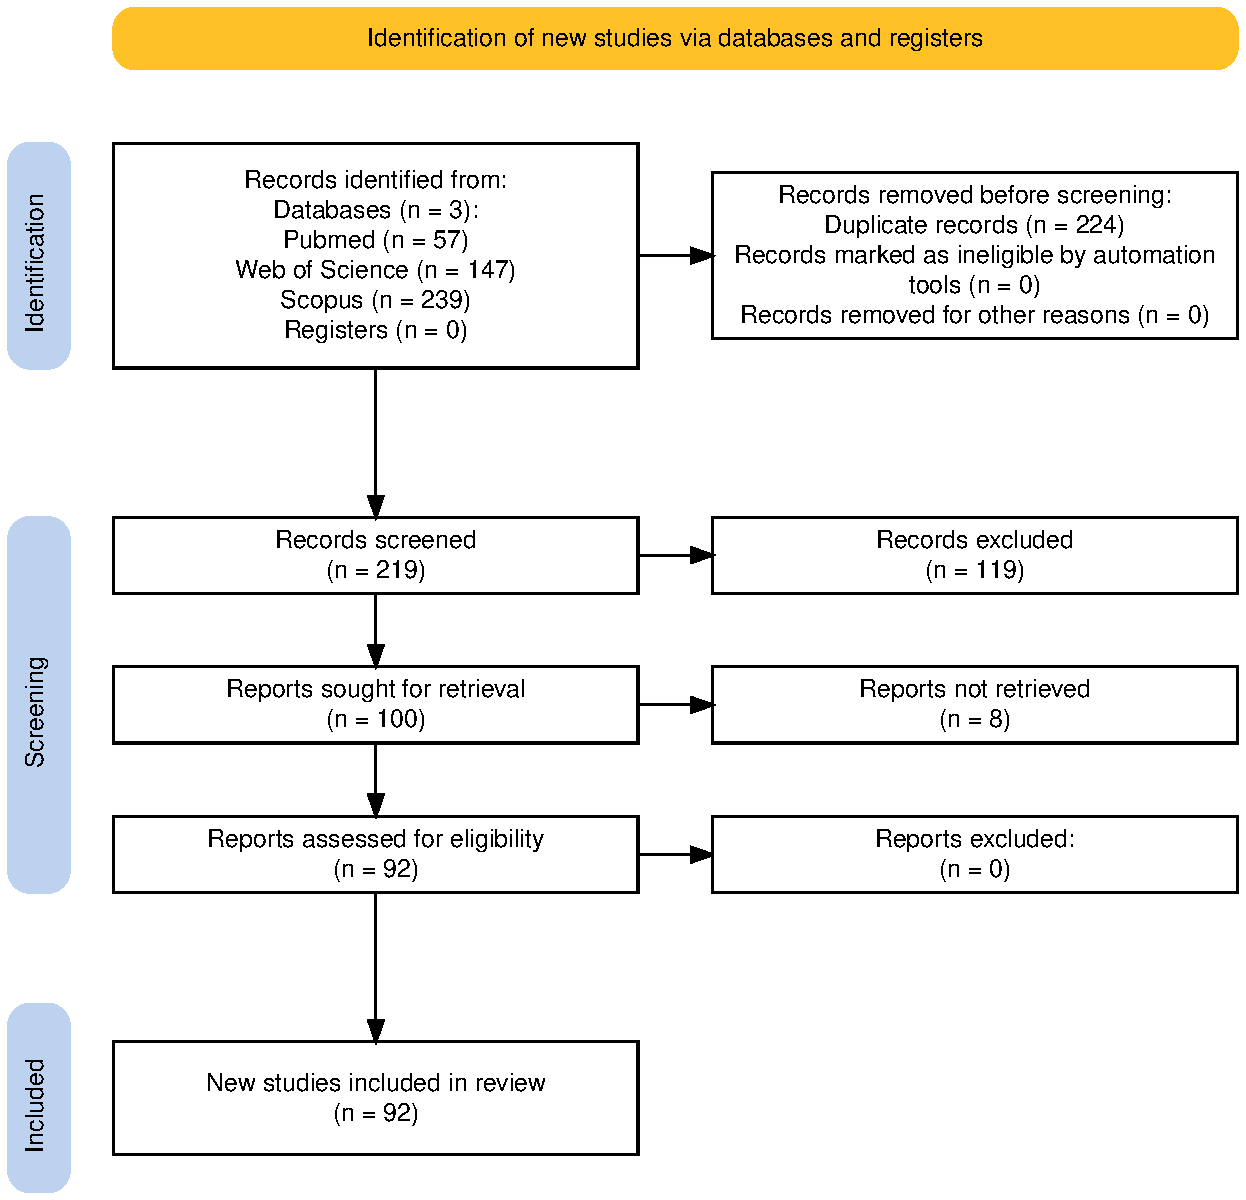
\includegraphics[width=\linewidth]{figures/prisma.pdf}
    \caption{PRISMA flow diagram for the present review.}
    \label{fig:prisma}
\end{figure}

Each of the 219 unique records underwent manual title-and-abstract screening against the following eligibility criteria.
A record was included if it met all of the following:
\begin{itemize}
    \item The study employed a neuroimaging modality (EEG, ERP, fNIRS, fMRI, MEG, ECoG, PET) or a non-invasive brain-stimulation modality (tDCS, tACS, TMS, GVS) to measure or modulate brain activity.
    \item The study addressed cybersickness or a closely related construct (visually induced motion sickness, simulator sickness, or motion sickness in a virtual environment) within a virtual reality or otherwise immersive context.
    \item The study reported original empirical data from human participants.
\end{itemize}

A record was excluded if it met any of the following:
\begin{itemize}
    \item The work was non-empirical (literature reviews, meta-analyses, editorials, letters, or conference abstracts without an accompanying full paper).
    \item The study did not address cybersickness or a related sickness construct as a primary outcome.
    \item The full text could not be retrieved.
\end{itemize}

Title-and-abstract screening excluded 119 records, leaving 100 reports sought for full-text retrieval.
Of these, 8 could not be obtained as full text and were excluded at the retrieval stage.
The remaining \textbf{92 articles} comprise the final corpus analysed in this review.

\subsection{Modalities and Dataset-Reuse Studies}
Two aspects of the corpus warrant explicit comment before the synthesis: the modalities that the query covered but that returned no eligible studies, and the inclusion of studies that rely on previously released datasets.

The query included PET, MEG, and fMRI terms alongside the more represented modalities.
PET returned no eligible studies; MEG returned a single record, which was excluded at the title-and-abstract stage as not addressing cybersickness or a related sickness construct; fMRI returned no records at all.
The absence of these modalities from the final corpus therefore reflects the current literature rather than a scope restriction imposed by the search.

A subset of retrieved studies train machine-learning classifiers on previously released datasets without recording new data.
Pure-dataset benchmarking is a related but methodologically distinct literature, since its primary objective is classification performance rather than the identification or modulation of neuromarkers.
Six papers in the final corpus reuse one or more publicly released datasets (in two cases combined with newly recorded data); they were retained because they satisfied all eligibility criteria and are flagged where relevant in the synthesis.

\subsection{Data Extraction and Thematic Synthesis}
For each of the 92 included articles, a structured data extraction process was performed.
This process was guided by a predefined protocol designed to ensure consistency and to facilitate subsequent comparison and synthesis.
The following data points were extracted from each paper:
\begin{enumerate}
    \item \textbf{Summary of Contribution:} A concise summary of the study's primary objective and its main contribution.
    \item \textbf{Sickness Measurement:} The methods used to measure or label cybersickness, distinguishing between subjective questionnaires (e.g., SSQ, FMS, VRSQ) and objective physiological or behavioural metrics (e.g., galvanic skin response, postural sway).
    \item \textbf{Methodological Pipeline:} A breakdown of the neurophysiological pipeline, including: (a) the measurement or stimulation modality, (b) the key feature extraction techniques (e.g., power spectral density, event-related potentials, functional connectivity), and (c) the primary analysis or classification methods (e.g., statistical tests, machine-learning models).
    \item \textbf{Theoretical Framework:} The explicitly stated or implicitly assumed theory of cybersickness (e.g., sensory conflict, postural instability) that guided the study's design or interpretation.
    \item \textbf{Quantitative Performance:} Reported performance measures, such as classification accuracy, correlation coefficients, root-mean-square error, or statistical significance values.
    \item \textbf{Empirical Study Details:} For empirical studies, specific details of the experimental protocol, including the VR environment, display hardware, sickness-inducing stimulus, and number of participants.
    \item \textbf{Reported Shortcomings:} Limitations, caveats, or weaknesses identified by the authors or apparent from the study's design.
\end{enumerate}

Following extraction, each paper was assigned to a primary research-objective category to support quantitative synthesis.
An initial set of categories was defined \textit{a priori} based on established research paradigms and refined iteratively during extraction.
The final categories, which structure the Results section, are: Classification (Binary, Likert, Continuous), Correlates (Brain Regions, Rhythms), Mitigation (A/B Testing, Real-time, Neurostimulation), User Differences, Dataset Provision, Recovery, and studies on the Effects of Cybersickness on other cognitive or performance metrics.
